\documentclass[11pt]{amsart}

\usepackage[T1]{fontenc}
\usepackage[utf8]{inputenc}
\usepackage{lmodern}
\usepackage{microtype}
\usepackage{amsmath,amssymb,amsthm,mathtools}
\usepackage{booktabs,array,tabularx,enumitem}
\usepackage{tikz}
\usetikzlibrary{positioning,calc}
\usepackage{xurl}
\usepackage[hidelinks]{hyperref}
\usepackage[nameinlink,capitalise,noabbrev]{cleveref}
\usepackage[a4paper,margin=30mm]{geometry}
\hypersetup{pdftitle={Tetrahedral Residuals, Affine 2-Torsion, and Double Pell Shells},pdfauthor={YUAN X},pdfsubject={Integral tetrahedral residuals, modular symmetry, Pell certificates, and conditional Ramanujan bounds},pdfkeywords={endpoint-sum map, affine 2-torsion, Pell equation, Ramanujan series, Lean 4}}

\newtheorem{theorem}{Theorem}[section]
\newtheorem{proposition}[theorem]{Proposition}
\newtheorem{lemma}[theorem]{Lemma}
\newtheorem{corollary}[theorem]{Corollary}
\theoremstyle{definition}
\newtheorem{definition}[theorem]{Definition}
\newtheorem{example}[theorem]{Example}
\theoremstyle{remark}
\newtheorem{remark}[theorem]{Remark}

\newcommand{\Z}{\mathbb Z}
\newcommand{\Q}{\mathbb Q}
\newcommand{\R}{\mathbb R}
\newcommand{\F}{\mathbb F}
\newcommand{\Aff}{\operatorname{Aff}}
\newcommand{\coker}{\operatorname{coker}}
\newcommand{\Tr}{\operatorname{Tr}}

\title[Tetrahedral residuals and double Pell shells]{Tetrahedral Residuals, Affine $2$-Torsion, and Double Pell Shells in a Four-Slice Six-Line Carrier}
\author{YUAN X}
\address{Enterprise Number Theory, independent research program}
\email{awdawmip@gmail.com}
\date{September 3, 2026}
\subjclass[2020]{05C50, 11D09, 11Y60, 15B36, 20C20, 68V20}
\keywords{signless incidence map, integral cokernel, affine plane, modular representation, Pell equation, Ramanujan series, Lean 4}

\begin{document}

\begin{abstract}
We study a finite carrier consisting of four overlapping three-line slices and six shared unoriented line families. Its incidence pattern is the vertex-edge incidence of $K_4$; a classical face-centred-cubic coordinate realization gives each slice three equal-length oriented vectors with pairwise angle $120$ degrees. On the zero-total vertex and edge lattices, the endpoint-sum map $\delta(v)_{ij}=v_i+v_j$ has a constructive integral cokernel
\[
 E_0/\delta(V_0)\simeq A_2(\Z)\oplus\Z/2\Z.
\]
We give explicit normal forms, an evenness criterion for lifting kernel states, and a Smith certificate with invariant factors $(1,1,2)$. After inverting $2$, the torsion disappears and only the two-dimensional $A_2$ residual remains. The tetrahedral $S_4$ action fixes the torsion line but admits no equivariant complement. Modulo $2$, the complete residual is naturally the space of affine functions on $\F_2^2$: its six nonconstant functions encode the six edges of $K_4$, while the nonzero constant exchanges opposite edges.

A separate arithmetic layer starts from the half-trace identity. If $(u+u^{-1})/2=P^2$, then the squared half-antitrace factors as $(P^2-1)(P^2+1)$, yielding paired positive and negative Pell shells. For $P=99$, exact identities involving $2,29,58,70,$ and $13$ organize the integers $396,9801,26390,$ and $1103$ appearing in Ramanujan's $N=58$ series. We do not derive the classical modular identity from these finite identities. Taking it as an external analytic input, we prove that reciprocal positive truncations decrease to $\pi$ from above and obtain the uniform ratio certificate $q_{58}=25/99^4$. The finite combinatorial, lattice, symmetry, Pell, monotonicity, and tail statements are accompanied by Lean 4 proof modules.
\end{abstract}

\maketitle

\section{Introduction and logical scope}

Ramanujan's celebrated series
\begin{equation}\label{eq:R58}
\frac1\pi=
\frac{2\sqrt2}{9801}
\sum_{n=0}^{\infty}
\frac{(4n)!}{(n!)^4}
\frac{1103+26390n}{396^{4n}}
\end{equation}
connects modular equations, complex multiplication, hypergeometric functions, and extremely rapid numerical convergence \cite{Ramanujan1914,BorweinBorwein1987,Berndt1994}. This article does not offer a new proof of \eqref{eq:R58}, nor does it replace the classical modular explanation. Its aim is narrower: to isolate exact finite structures that can be proved independently of the modular identity and to state precisely where the external analytic input enters.

There are two main layers.

The first is a tetrahedral lattice problem. Four slices meet pairwise in six line families, giving the complete graph $K_4$. Zero-sum slice potentials are sent to line states by endpoint addition. Over the integers the quotient retains a single parity class; over any coefficient field in which $2$ is invertible, that class disappears. The tetrahedral symmetry does not split into a product action on the free and torsion coordinates. Instead, the hidden Klein four subgroup acts by translations of the torsion fibre.

The second is an arithmetic certificate. A square half-trace forces a fourth-power residual $P^4-1$, which factors into positive and negative Pell shells. At $P=99$ these shells reproduce a network of exact identities among the conspicuous integers in \eqref{eq:R58}. Once \eqref{eq:R58} itself is assumed, positivity and a uniform term-ratio bound give monotonic reciprocal approximants and an explicit tail estimate.

The principal finite conclusions are summarized below.

\begin{theorem}[Structural summary]\label{thm:summary}
For the four-slice six-line carrier described in \cref{sec:carrier}:
\begin{enumerate}[label=\textup{(\roman*)}]
\item the integral zero-total residual quotient is
\[
 E_0/\delta(V_0)\simeq A_2(\Z)\oplus\Z/2\Z;
\]
\item after scalar extension to a field $K$ of characteristic different from $2$,
\[
 E_0(K)/\delta(V_0(K))\simeq A_2(K);
\]
\item modulo $2$, the residual is the non-split $S_4$-module
\[
 \Aff(\F_2^2,\F_2),
\]
with invariant constant line and no $S_4$-equivariant retraction onto that line;
\item if an invertible parameter $u$ has half-trace $P^2$, then its half-antitrace satisfies
\[
 \left(\frac{u-u^{-1}}2\right)^2=(P^2-1)(P^2+1);
\]
\item assuming Ramanujan's identity \eqref{eq:R58}, the reciprocal truncations decrease strictly to $\pi$ from above, and the omitted tail is controlled by
\[
 q_{58}=\frac{25}{99^4}<1.
\]
\end{enumerate}
\end{theorem}

The lattice quotient belongs to the general study of integral incidence matrices and signless Laplacians \cite{CvetkovicRowlinsonSimic2007,Newman1972}. The characteristic-two module is a concrete form of the augmentation module for the permutation action of $S_4$ on four points, a classical modular representation \cite{Benson1991,JamesKerber1981}. Our contribution is therefore not the invention of those general objects. It is the simultaneous constructive normal form, explicit cocycle and nonsplitting computation, affine support interpretation, arithmetic shell comparison, and machine-checkable packaging in one small model.

\section{The four-slice six-line carrier}\label{sec:carrier}

\subsection{Incidence and the tetrahedron}

Let the slices be $A,B,C,D$ and the six unoriented line families be $L_1,\dots,L_6$, with incidence table
\[
\begin{array}{c|c}
\text{slice}&\text{line families}\\ \hline
A&L_1,L_3,L_6\\
B&L_1,L_4,L_5\\
C&L_2,L_3,L_5\\
D&L_2,L_4,L_6
\end{array}
\]
Thus
\[
 L_1=AB,\quad L_2=CD,\quad L_3=AC,\quad
 L_4=BD,\quad L_5=BC,\quad L_6=AD.
\]

\begin{proposition}[Exact $K_4$ incidence]\label{prop:k4}
Every slice contains three line families, every line family belongs to two slices, and every pair of distinct slices shares exactly one line family. The map taking a line family to the two slices containing it is a bijection with the six edges of $K_4$.
\end{proposition}

\begin{proof}
The row and column counts are immediate from the table. Its six columns give six distinct two-element subsets of a four-element set, hence all of them.
\end{proof}

\begin{center}
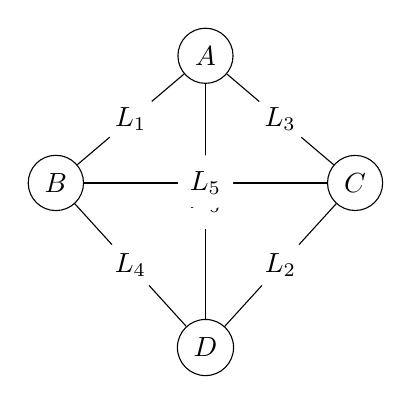
\begin{tikzpicture}[scale=0.95,every node/.style={circle,draw,minimum size=7mm,font=\bfseries}]
\node (A) at (0,2.4) {$A$};
\node (B) at (-2,0.7) {$B$};
\node (C) at (2,0.7) {$C$};
\node (D) at (0,-1.5) {$D$};
\draw (A)--node[draw=none,fill=white,inner sep=1pt] {$L_1$} (B);
\draw (A)--node[draw=none,fill=white,inner sep=1pt] {$L_3$} (C);
\draw (A)--node[draw=none,fill=white,inner sep=1pt] {$L_6$} (D);
\draw (B)--node[draw=none,fill=white,inner sep=1pt] {$L_5$} (C);
\draw (B)--node[draw=none,fill=white,inner sep=1pt] {$L_4$} (D);
\draw (C)--node[draw=none,fill=white,inner sep=1pt] {$L_2$} (D);
\end{tikzpicture}
\end{center}

\subsection{An FCC coordinate realization}

In $\Z^3$, take the six unoriented representatives
\begin{align*}
\ell_1&=(1,1,0), & \ell_2&=(1,-1,0),\\
\ell_3&=(1,0,1), & \ell_4&=(1,0,-1),\\
\ell_5&=(0,1,1), & \ell_6&=(0,1,-1).
\end{align*}
Choose the oriented triples
\[
\begin{array}{c|c}
A&(\ell_1,-\ell_3,-\ell_6)\\
B&(\ell_1,-\ell_4,-\ell_5)\\
C&(\ell_2,-\ell_3,\ell_5)\\
D&(\ell_2,-\ell_4,\ell_6).
\end{array}
\]

\begin{proposition}[Local $120$-degree certificate]\label{prop:120}
In every oriented triple, the three vectors sum to zero, each vector has squared length $2$, and every two distinct vectors have inner product $-1$. Hence every pair makes an angle of $120$ degrees.
\end{proposition}

\begin{proof}
All statements follow by direct substitution. Equal squared length $2$ and inner product $-1$ give normalized cosine $-1/2$.
\end{proof}

This realization is used only as a computable carrier model. No ontological identification of these six lines with a complete ambient geometry is asserted.

\section{The integral tetrahedral residual}\label{sec:integral}

Order the edges as
\[
 (AB,AC,AD,BC,BD,CD).
\]
Define
\[
 V_0=\{v\in\Z^4:v_A+v_B+v_C+v_D=0\},
\]
\[
 E_0=\{x\in\Z^6:\textstyle\sum_e x_e=0\},
\]
and
\[
\delta(v)=
(v_A+v_B,v_A+v_C,v_A+v_D,v_B+v_C,v_B+v_D,v_C+v_D).
\]
Since every vertex occurs on three edges,
\[
 \sum_e\delta(v)_e=3\sum_i v_i,
\]
so $\delta(V_0)\subset E_0$.

Define the opposite-edge sums
\begin{align*}
 m_0(x)&=x_{AB}+x_{CD},\\
 m_1(x)&=x_{AC}+x_{BD},\\
 m_2(x)&=x_{AD}+x_{BC}.
\end{align*}
On $E_0$, their sum is zero, so
\[
 m(x)=(m_0,m_1,m_2)\in A_2(\Z)
 =\{(p,q,r)\in\Z^3:p+q+r=0\}.
\]
They vanish on $\delta(V_0)$.

If $m(x)=0$, then uniquely
\[
 x=K(a,b,c):=(a,b,c,-c,-b,-a).
\]

\begin{theorem}[Parity lifting criterion]\label{thm:lift}
There exists $v\in V_0$ with $\delta(v)=K(a,b,c)$ if and only if $a+b+c$ is even.
\end{theorem}

\begin{proof}
If $K(a,b,c)=\delta(v)$, then
\[
 a+b+c=3v_A+(v_B+v_C+v_D)=2v_A.
\]
Conversely, if $a+b+c=2t$, then
\[
 v=(t,a-t,b-t,c-t)
\]
has zero total and maps to $K(a,b,c)$.
\end{proof}

Thus
\[
 \tau=K(1,0,0)=(1,0,0,0,0,-1)
\]
is nonliftable, while $2\tau$ lifts.

Define the star parity
\[
 \chi_A(x)=x_{AB}+x_{AC}+x_{AD}\pmod2.
\]
For $p,q\in\Z$ and $\varepsilon\in\{0,1\}$, set
\[
 N(p,q,\varepsilon)
 = (\varepsilon,0,0,-p-q,q,p-\varepsilon).
\]
Then
\[
 m(N)=(p,q,-p-q),\qquad \chi_A(N)=\varepsilon.
\]

\begin{theorem}[Integral normal form]\label{thm:normal}
The map
\[
 \Phi:E_0\to A_2(\Z)\oplus\F_2,
 \qquad \Phi(x)=(m(x),\chi_A(x)),
\]
is surjective with kernel $\delta(V_0)$. Consequently
\[
 \boxed{E_0/\delta(V_0)\simeq A_2(\Z)\oplus\Z/2\Z.}
\]
Every class has a unique representative coordinate $(p,q,\varepsilon)$ through $N(p,q,\varepsilon)$.
\end{theorem}

\begin{proof}
The normal forms prove surjectivity. Every image $\delta(v)$ has zero opposite-edge sums and even star sum. Conversely, if both invariants vanish, then $x=K(a,b,c)$ with $a+b+c$ even, so \cref{thm:lift} supplies a lift. Uniqueness follows because the opposite-edge sums determine $p,q$, and the star parity determines $\varepsilon$.
\end{proof}

\subsection{Smith invariant certificate}

In difference bases of $V_0$ and the first-five-coordinate basis of $E_0$, the restricted map is
\[
D=\begin{pmatrix}
0&1&0\\
1&-1&1\\
1&0&-1\\
0&-1&0\\
-1&1&-1
\end{pmatrix}.
\]
It contains a unit entry, a $2\times2$ minor equal to $-1$, and its ten maximal minors are
\[
(2,0,0,0,2,0,-2,0,0,2).
\]
Hence its nonzero Smith invariant factors are $(1,1,2)$, independently confirming
\[
 \coker D\simeq\Z^2\oplus\Z/2\Z.
\]

\section{Scalar extension and metric normalization}\label{sec:scalar}

Let $K$ be a field of characteristic different from $2$. For $x\in E_0(K)$ define
\[
 P(x)=\left(\frac{m_0}2,\frac{m_1}2,\frac{m_2}2,
             \frac{m_2}2,\frac{m_1}2,\frac{m_0}2\right).
\]
The state $P(x)$ is constant on opposite pairs and has the same $m$-coordinate as $x$. Thus $r=x-P(x)=K(a,b,c)$, and division by $2$ gives a potential lifting $r$.

\begin{theorem}[Continuous splitting]\label{thm:continuous}
For every field $K$ with $\operatorname{char}K\ne2$,
\[
 E_0(K)/\delta(V_0(K))\simeq A_2(K)\simeq K^2.
\]
The integral torsion generator becomes zero after scalar extension.
\end{theorem}

\begin{proof}
The decomposition $x=P(x)+\delta(v)$ shows that the residual is determined by $m(x)$. Every $A_2(K)$ coordinate has an opposite-pair-constant representative. Finally,
\[
 \left(\frac12,\frac12,-\frac12,-\frac12\right)
\]
is a zero-sum potential mapping to $\tau$.
\end{proof}

A convenient basis of the continuous residual plane is
\[
 u=\left(\frac12,-\frac12,0,\frac12,-\frac12,0\right),\qquad
 w=\left(\frac12,0,-\frac12,\frac12,0,-\frac12\right),
\]
after grouping opposite pairs. Its Gram matrix is
\[
G_{\mathrm{proj}}=\begin{pmatrix}1&1/2\\1/2&1\end{pmatrix},
\qquad \det G_{\mathrm{proj}}=\frac34.
\]
The integral intersection basis $2u,2w$ has Gram matrix
\[
G_{\mathrm{int}}=\begin{pmatrix}4&2\\2&4\end{pmatrix},
\qquad \det G_{\mathrm{int}}=12.
\]
The squared covolume ratio is $16$, so the lattice index in this projected plane is $4$. This index compares two free lattices and should not be confused with the single $\Z/2$ class in the five-dimensional cokernel.

\section{Tetrahedral symmetry and non-splitting}\label{sec:symmetry}

Every permutation of $A,B,C,D$ permutes the six edges and satisfies
\[
 \sigma_E(\delta(v))=\delta(\sigma_V(v)).
\]
Thus $S_4$ acts on the residual group. For the adjacent transpositions
\[
 s_1=(AB),\qquad s_2=(BC),\qquad s_3=(CD),
\]
the normal coordinates transform as
\begin{equation}\label{eq:actions}
\begin{aligned}
 s_1(p,q,\varepsilon)&=(p,-p-q,\varepsilon+\bar p),\\
 s_2(p,q,\varepsilon)&=(q,p,\varepsilon),\\
 s_3(p,q,\varepsilon)&=(p,-p-q,\varepsilon),
\end{aligned}
\end{equation}
where $\bar p$ is the parity of $p$.

Modulo $2$, write $W=\F_2^3$ with coordinates $(p,q,e)$. Then
\begin{equation}\label{eq:mod2}
\begin{aligned}
 s_1(p,q,e)&=(p,p+q,e+p),\\
 s_2(p,q,e)&=(q,p,e),\\
 s_3(p,q,e)&=(p,p+q,e).
\end{aligned}
\end{equation}
These maps satisfy all Coxeter relations for $S_4$.

The free $A_2$ coordinate only sees the permutation of the three opposite-edge matchings, so the action factors through $S_4\twoheadrightarrow S_3$. The kernel is
\[
 V_4=\{1,(AB)(CD),(AC)(BD),(AD)(BC)\}.
\]
Its three nonidentity elements act on $W$ by
\begin{align*}
 (AB)(CD):(p,q,e)&\mapsto(p,q,e+p),\\
 (AC)(BD):(p,q,e)&\mapsto(p,q,e+q),\\
 (AD)(BC):(p,q,e)&\mapsto(p,q,e+p+q).
\end{align*}
Thus the invisible rotations pair perfectly with the three nonzero linear functionals on the free parity plane.

Let
\[
 t=(0,0,1),\qquad P=(1,0,0),\qquad Q=(0,1,0).
\]
The line $T=\langle t\rangle$ is fixed pointwise.

\begin{theorem}[$S_4$ non-splitting]\label{thm:nonsplit}
There is no $S_4$-invariant additive retraction $r:W\to\F_2$ with $r(t)=1$. Equivalently, the invariant torsion line $T$ has no $S_4$-equivariant complement.
\end{theorem}

\begin{proof}
If such $r$ existed, $s_2(P)=Q$ would imply $r(P)=r(Q)$. Since $s_3(P)=P+Q$, invariance would then imply $r(Q)=0$ and hence $r(P)=0$. But $s_1(P)=P+Q+t$ would give
\[
 0=r(P)=r(P)+r(Q)+r(t)=1,
\]
a contradiction.
\end{proof}

\section{The affine plane over $\F_2$}\label{sec:affine}

Label the four vertices by
\[
 A=(0,0),\quad B=(1,0),\quad C=(0,1),\quad D=(1,1)
\]
in $\mathbb A=\F_2^2$. Associate to $(p,q,e)\in W$ the affine function
\[
 f_{p,q,e}(x,y)=e+px+qy.
\]

\begin{theorem}[Affine-function model]\label{thm:affine}
The map
\[
 W\longrightarrow\Aff(\F_2^2,\F_2),\qquad
 (p,q,e)\longmapsto f_{p,q,e},
\]
is an $S_4$-equivariant linear isomorphism, using $S_4\simeq\operatorname{AGL}(2,2)$. The supports of the six nonconstant affine functions are exactly the six edges of $K_4$. Addition of $t$ takes a support to its complement and therefore exchanges opposite edges.
\end{theorem}

\begin{proof}
Affine functions are uniquely determined by $(p,q,e)$, so the map is a linear isomorphism. The affine group of the four-point plane has order $4\cdot6=24$ and acts faithfully, hence is $S_4$. Direct precomposition gives the generator formulas \eqref{eq:mod2}. If $(p,q)\ne(0,0)$, the two level sets of $px+qy$ each contain two points. The three nonzero linear parts $x,y,x+y$ give the complementary pairs
\[
 AC\leftrightarrow BD,\qquad
 AB\leftrightarrow CD,\qquad
 AD\leftrightarrow BC.
\]
Adding the constant $1$ exchanges the two level sets.
\end{proof}

The free parity coordinate selects one of the three perfect matchings, and the torsion bit selects one of its two edges. Thus the factorization $6=3\cdot2$ is structural rather than merely numerical.

\section{Square half-trace and double Pell shells}\label{sec:pell}

Let $K$ be a field of characteristic different from $2$ and let $u\in K^\times$. Define
\[
 H(u)=\frac{u+u^{-1}}2,\qquad
 A(u)=\frac{u-u^{-1}}2.
\]
Direct expansion gives
\[
 H(u)^2-A(u)^2=1.
\]

\begin{theorem}[Square half-trace splitting]\label{thm:halftrace}
If $H(u)=P^2$, then
\[
 A(u)^2=P^4-1=(P^2-1)(P^2+1).
\]
If, in addition,
\[
 P^2-d_+y_+^2=1,\qquad
 P^2-d_-y_-^2=-1,
\]
then
\[
 d_+d_-(y_+y_-)^2=P^4-1.
\]
\end{theorem}

\begin{proof}
The first identity follows from $H^2-A^2=1$ and the difference of squares. The two Pell equations give $d_+y_+^2=P^2-1$ and $d_-y_-^2=P^2+1$; multiplying proves the second identity.
\end{proof}

Inversion $u\mapsto u^{-1}$ fixes $H$ and negates $A$. Thus the symmetric coordinate controls the common fourth residual, while the sign of the antitrace retains orientation information.

\section{The $P=99$ arithmetic certificate}\label{sec:n58}

Take
\[
 P=99,
 \qquad(d_+,y_+)=(2,70),
 \qquad(d_-,y_-)=(58,13).
\]
Then
\[
 99^2-2\cdot70^2=1,
 \qquad
 99^2-58\cdot13^2=-1.
\]
Consequently
\[
 2\cdot58\,(70\cdot13)^2=99^4-1.
\]
The companion relation
\[
 70^2-29\cdot13^2=-1
\]
and the equality $2\cdot58=4\cdot29$ combine into
\[
 \boxed{9801^2-29\cdot1820^2=1,}
\]
where
\[
 9801=99^2,\qquad 1820=2\cdot70\cdot13.
\]
The remaining integer certificates are
\[
 396=4\cdot99,
\]
\[
 26390=29\cdot70\cdot13,
\]
and
\[
 \boxed{4\cdot1103
 =29\cdot70\cdot13-2\cdot99(99+13-1).}
\]
These identities place the four familiar integers in one arithmetic diagram. They do not by themselves prove the modular-hypergeometric identity \eqref{eq:R58}.

The small fourth-power parameter is
\[
 z=99^{-4}=\frac1{96059601},
\]
and the series base satisfies
\[
 \frac1{396^4}=\frac1{4^4}\,z=\frac1{256}\,z.
\]

\section{A conditional precision theorem}\label{sec:precision}

Define
\[
 a_n=\frac{(4n)!}{(n!)^4}
 \frac{1103+26390n}{396^{4n}},
 \qquad
 C=\frac{2\sqrt2}{9801},
\]
\[
 S_M=C\sum_{n=0}^M a_n,
 \qquad
 \Pi_M=\frac1{S_M}.
\]
In this section only, Ramanujan's identity \eqref{eq:R58} is assumed as an external theorem.

The exact successive-term ratio is
\[
\frac{a_{n+1}}{a_n}
=
\frac{(4n+1)(4n+2)(4n+3)(4n+4)}{(n+1)^4}
\frac{1103+26390(n+1)}{1103+26390n}
\frac1{396^4}.
\]
The factorial factor is at most $4^4=256$, while
\[
 \frac{1103+26390(n+1)}{1103+26390n}<25.
\]
Therefore
\[
 0<\frac{a_{n+1}}{a_n}
 \le\frac{6400}{396^4}
 =\frac{25}{99^4}
 =:q_{58}<1.
\]
Numerically,
\[
 q_{58}=2.6025508892130418\ldots\times10^{-7}.
\]

\begin{theorem}[Conditional monotone approximation and tail bound]\label{thm:precision}
Assume \eqref{eq:R58}. Then $S_M$ is strictly increasing with $0<S_M<1/\pi$, and $\Pi_M$ is strictly decreasing with $\Pi_M>\pi$. If
\[
 R_M=\frac1\pi-S_M=C\sum_{n=M+1}^\infty a_n,
\]
then
\[
 0<R_M\le\frac{Ca_{M+1}}{1-q_{58}}.
\]
Moreover,
\[
 \Pi_M-\pi=\frac{\pi R_M}{S_M},
\]
and
\[
 \frac{\Pi_M}{\pi}-1
 =\frac{R_M}{S_M}
 \le\frac{Ca_{M+1}}{(1-q_{58})S_M}.
\]
\end{theorem}

\begin{proof}
All terms are positive, so the partial sums are strictly increasing. The assumed identity places every finite partial sum below $1/\pi$, and taking reciprocals reverses the inequality. The ratio bound implies inductively
\[
 a_{M+1+j}\le q_{58}^j a_{M+1}.
\]
Summing the geometric majorant gives the tail estimate. Finally,
\[
 \frac1{S_M}-\frac1{S_M+R_M}
 =\frac{R_M}{S_M(S_M+R_M)}
 =\frac{\pi R_M}{S_M},
\]
because $S_M+R_M=1/\pi$.
\end{proof}

For illustration,
\[
\begin{array}{c|c|c}
M&\Pi_M&\Pi_M-\pi\ \text{(order)}\\ \hline
0&3.1415927300133056603&7.64\times10^{-8}\\
1&3.1415926535897938780&6.40\times10^{-16}\\
2&3.1415926535897932384626491&5.68\times10^{-24}\\
3&3.1415926535897932384626433832795553&5.24\times10^{-32}
\end{array}
\]
Every listed truncation lies above $\pi$, as required.

\section{Finite generating lifts and majorization}\label{sec:majorization}

Let $K$ be a field of characteristic zero, let $s_n,t_n$ be nonzero coefficient channels, and let $\lambda\ne0$. Define
\[
 P_n=\lambda\frac{s_n}{nt_n},\qquad n\ge1.
\]
Then
\[
 s_n=\lambda^{-1}nt_nP_n.
\]
Multiplication by an arbitrary response factor $r_nz^n$ and finite summation give the exact identity
\[
 \sum_{n=1}^M s_nr_nz^n
 =\sum_{n=1}^M\lambda^{-1}nt_nP_nr_nz^n.
\]
This is purely algebraic; analytic hypotheses enter only when one passes to infinite series.

A second finite certificate compares the decreasing vectors
\[
 \mathbf a=\left(1,\frac34,\frac12,\frac14,0\right),
 \qquad
 \mathbf b=\left(\frac56,\frac46,\frac36,\frac26,\frac16\right).
\]
Their total sums agree and the prefix differences are
\[
 0,\frac16,\frac14,\frac14,\frac16,0.
\]
Thus $\mathbf a$ strictly majorizes $\mathbf b$.

More generally, for integers $k,m\ge1$, let
\[
 a_i=\frac{k-i}{k},\qquad
 b_i=\frac{k+m-i}{k+2m},\qquad 0\le i\le k.
\]
For $1\le r\le k$,
\[
 \sum_{i=0}^{r-1}a_i-\sum_{i=0}^{r-1}b_i
 =\frac{mr(k-r+1)}{k(k+2m)}>0,
\]
while the full sums are equal. Karamata's inequality \cite{HardyLittlewoodPolya1952,MarshallOlkinArnold2011} therefore gives, for every strictly concave $f$,
\[
 \sum_i f(a_i)<\sum_i f(b_i).
\]
Taking $f(x)=\log(n+x)$ for $n>0$ yields
\[
 \prod_{i=0}^k(n+a_i)<\prod_{i=0}^k(n+b_i).
\]
This is the finite rational skeleton needed in comparisons of shifted factorial or Gamma factors. A complete $\log\Gamma$ bridge is not claimed here.

\section{Formal verification boundary}\label{sec:lean}

The development was divided into two Lean 4 branches so that finite residual geometry and arithmetic certificates could be checked independently.

The residual and symmetry branch contains modules for:
\begin{itemize}[leftmargin=2em]
\item the four-slice six-line kernel and parity witness;
\item exact integral equivalence and unique normal forms;
\item real scalar extension and torsion loss;
\item $K_4$ covariance under all slice permutations;
\item adjacent transpositions, Coxeter relations, the hidden Klein-four action, and the nonsplitting theorem.
\end{itemize}
The strict warning-fatal run succeeded at commit
\[
\texttt{95a9cd418f6abdb4916f5cf8182437af61dba9db}.
\]

The arithmetic and analytic-certificate branch contains modules for:
\begin{itemize}[leftmargin=2em]
\item FCC incidence and local $120$-degree certificates;
\item Smith invariant factors, rational splitting, and residual metrics;
\item half-trace algebra and double Pell fusion;
\item the $P=99$ integer identities;
\item finite generating lifts and majorization arithmetic;
\item positive reciprocal monotonicity and geometric tail bounds, including $q_{58}$.
\end{itemize}
The aggregate command
\begin{verbatim}
lake build --wfail -KCI EnterpriseMath
\end{verbatim}
succeeded at commit
\[
\texttt{ca2b30c7ef45b470d0d5cb6955def48610cd9dd7}.
\]
No \texttt{sorry}, \texttt{admit}, or custom axiom is used in the listed paper modules. The classical identity \eqref{eq:R58} is not replaced by the finite Lean development; it remains the explicit external assumption in \cref{thm:precision}. Background on Lean and mathlib appears in \cite{deMouraEtAl2015,Mathlib2020}.

\section{Boundaries and conclusion}

The finite carrier supports three compatible but logically distinct chains:
\[
 K_4\text{ carrier}
 \longrightarrow A_2(\Z)\oplus C_2
 \longrightarrow
 \begin{cases}
 A_2(\R),&\text{after inverting }2,\\
 \Aff(\F_2^2,\F_2),&\text{after reduction mod }2,
 \end{cases}
\]
\[
 \text{square half-trace}
 \longrightarrow(P^2-1)(P^2+1)
 \longrightarrow\text{paired Pell shells},
\]
and, only after importing the classical modular identity,
\[
 \text{positive Ramanujan series}
 \longrightarrow\Pi_M\downarrow\pi
 \quad\text{with an explicit tail bound}.
\]

Several boundaries are essential. The FCC vectors provide a coordinate realization, not a proof that the six lines exhaust an ambient space. The Pell identities organize exact integers but do not derive the modular transformation behind \eqref{eq:R58}. The affine model is a complete finite proof, while only part of that presentation has been packaged into the strict Lean workflow. Finally, the classical Ramanujan formula is not claimed as a new result.

The next natural problems are to formalize the affine-function equivalence itself, to classify analogous zero-sum signless-incidence cokernels for larger graphs, and to determine whether any rigorous functorial construction links the characteristic-two fibre phase to signed Pell-shell choices without confusing arithmetic certificates with modular-form proofs.

\section*{Data, code, and artificial-intelligence disclosure}

The Lean code is publicly available in the \emph{Enterprise Math} repository on the branches
\path{formalization/precision-pi-paper-ii-kernel-v1} and
\path{formalization/precision-pi-paper-ii-v3}. Exact certified commits and build commands are stated in \cref{sec:lean}.

OpenAI's ChatGPT assisted with translation, language editing, organization of the exposition, literature discovery, numerical cross-checking, and parts of the Lean proof-development workflow. It is not an author. The named author assumes full responsibility for the mathematical content, citations, and dissemination of this manuscript.

\begin{thebibliography}{99}

\bibitem{Benson1991}
D.~J. Benson,
\emph{Representations and Cohomology I: Basic Representation Theory of Finite Groups and Associative Algebras},
Cambridge Studies in Advanced Mathematics, vol.~30, Cambridge University Press, Cambridge, 1991.

\bibitem{Berndt1994}
B.~C. Berndt,
\emph{Ramanujan's Notebooks, Part IV},
Springer-Verlag, New York, 1994.

\bibitem{BorweinBorwein1987}
J.~M. Borwein and P.~B. Borwein,
\emph{Pi and the AGM: A Study in Analytic Number Theory and Computational Complexity},
Wiley, New York, 1987.

\bibitem{CvetkovicRowlinsonSimic2007}
D. Cvetkovi\'c, P. Rowlinson, and S. Simi\'c,
Signless Laplacians of finite graphs,
\emph{Linear Algebra Appl.} \textbf{423} (2007), 155--171.

\bibitem{deMouraEtAl2015}
L. de Moura, S. Kong, J. Avigad, F. van Doorn, and J. von Raumer,
The Lean theorem prover (system description),
in \emph{Automated Deduction -- CADE-25}, Lecture Notes in Computer Science, vol.~9195, Springer, 2015, pp.~378--388.

\bibitem{HardyLittlewoodPolya1952}
G.~H. Hardy, J.~E. Littlewood, and G. P\'olya,
\emph{Inequalities}, 2nd ed., Cambridge University Press, Cambridge, 1952.

\bibitem{JamesKerber1981}
G. James and A. Kerber,
\emph{The Representation Theory of the Symmetric Group},
Encyclopedia of Mathematics and its Applications, vol.~16, Addison-Wesley, Reading, MA, 1981.

\bibitem{MarshallOlkinArnold2011}
A.~W. Marshall, I. Olkin, and B.~C. Arnold,
\emph{Inequalities: Theory of Majorization and Its Applications}, 2nd ed.,
Springer, New York, 2011.

\bibitem{Mathlib2020}
The mathlib Community,
The Lean mathematical library,
in \emph{Proceedings of the 9th ACM SIGPLAN International Conference on Certified Programs and Proofs}, ACM, 2020, pp.~367--381.

\bibitem{Newman1972}
M. Newman,
\emph{Integral Matrices},
Pure and Applied Mathematics, vol.~45, Academic Press, New York, 1972.

\bibitem{Ramanujan1914}
S. Ramanujan,
Modular equations and approximations to $\pi$,
\emph{Quart. J. Pure Appl. Math.} \textbf{45} (1914), 350--372.

\end{thebibliography}

\end{document}
